\documentclass[11pt,a4paper]{article}

\usepackage[left=2.2cm,right=3.0cm,top=2.4cm,bottom=2.6cm,
            marginparwidth=2.15cm,marginparsep=3mm]{geometry}
\usepackage{amsmath,amssymb,mathtools}
\usepackage{booktabs}
\usepackage{rotating}
\usepackage[font=small]{caption}
\usepackage[font=small]{subcaption}
\usepackage{tikz}
\usepackage{pgfplots}
\pgfplotsset{compat=1.18}
\usetikzlibrary{arrows.meta,calc,decorations.pathreplacing}
\usepackage[colorlinks=true,allcolors=blue!55!black]{hyperref}
\providecommand{\mathdefault}[1]{#1}   %% required by matplotlib's pgf output

%% float placement: the defaults are far too strict for a document with this many
%% figures, and a single deferred float blocks every later one
\renewcommand{\topfraction}{0.9}
\renewcommand{\bottomfraction}{0.7}
\renewcommand{\textfraction}{0.07}
\renewcommand{\floatpagefraction}{0.75}
\setcounter{topnumber}{3}
\setcounter{totalnumber}{4}

%% axial lengths carry the symbol L, diameters the symbol D
\newcommand{\Lpet}{L_{\mathrm{PET}}}
\newcommand{\Lsrc}{L_{\mathrm{s}}}
\newcommand{\Lmrd}{L_{\mathrm{MRD}}}
\newcommand{\Dpet}{D_{\mathrm{PET}}}
\newcommand{\Dcyl}{D_{\mathrm{cyl}}}
\newcommand{\Sid}{S_{\mathrm{ideal}}}
\newcommand{\Snema}{S_{\mathrm{NEMA}}}
\newcommand{\Fo}{F_{\mathrm{o}}}
\newcommand{\Ft}{F_{t}}
\newcommand{\Fy}{F_{y}}
\newcommand{\Fz}{F_{z}}
\newcommand{\rT}{r_{\mathrm{TOF}}}
\newcommand{\rN}{r_{\mathrm{nonTOF}}}
\newcommand{\so}{\sigma_{\!o}}
\newcommand{\kf}{(8\ln 2)^{3/2}}
\newcommand{\Lex}{\Lambda}
\newcommand{\vt}{\sigma_t^{2}+\so^{2}}
\newcommand{\vy}{\sigma_y^{2}+\so^{2}}
\newcommand{\vz}{\sigma_z^{2}+\so^{2}}
\newcommand{\marginnotefont}{\scriptsize\raggedright}
\DeclarePairedDelimiter{\abs}{\lvert}{\rvert}

\title{Comparing short and long PET systems on a resolution-dependent task}
\author{Johan Nuyts, Seyed Amir Zamanpour, Georg Schramm}
\date{\today}

%% ---------------------------------------------------------------------------
%% Files, all expected in this directory:
%%   main.tex                    this file (text, equations, captions)
%%   tikz-slog.tex               Figure 1  (TikZ + pgfplots)
%%   tikz-geometry.tex           Figure 2  (TikZ)
%%   tikz-regimes.tex            Figure 3  (TikZ, both rows)
%%   fig-slog2d.pdf              Figure 1   \
%%   fig-profile.pgf             Figure 4    |  written by make_all.py,
%%   fig-ripple.pgf              Figure 5    |  which drives the modules in
%%   fig-beds.pgf                Figure 6    |  paper/ on top of the slogpet
%%   fig-scenarios.pgf           Figure 7    |  package
%%   table.tex                   Table 2    /
%% Build with:  python3 ../make_all.py  &&  latexmk -pdf main.tex
%% (make_all.py lives in the repository root and writes its output here)
%% ---------------------------------------------------------------------------

%% tikz-regimes.tex --- included by sensitivity_derivation.tex
%% Macros for Figure 2 (three regimes of the ring-difference limit):
%%   \regimecyl{A}{L}{A_MRD/2}    top row:    cylinder, line source, acceptance wedges
%%   \branchpanel{A}{L}{A_MRD/2}  bottom row: the profile d_1(z) that is integrated
%% Both use the same horizontal unit and the same bounding box in z, so a column of
%% the two pictures is registered: the blue curve below is the envelope of the wedges
%% above it. Pass any value >= A/2 as the third argument to disable the cap.
%% Requires: tikz, arrows.meta.

%% common horizontal extent, in the same units as z
\newcommand{\rgLeft}{-6.0}
\newcommand{\rgRight}{6.6}

\newcommand{\regimecyl}[3]{%
  \pgfmathsetmacro{\rA}{#1}\pgfmathsetmacro{\rL}{#2}\pgfmathsetmacro{\rM}{#3}
  \pgfmathsetmacro{\rAh}{\rA/2}\pgfmathsetmacro{\rLh}{\rL/2}
  \pgfmathsetmacro{\rR}{2.2}\pgfmathsetmacro{\rt}{0.30}
  \pgfmathsetmacro{\re}{0.58}\pgfmathsetmacro{\reo}{\re*(\rR+\rt)/\rR}
\begin{tikzpicture}[x=0.40cm,y=0.40cm,>={Latex[length=1.4mm]}]
  % ---- detector cylinder ----------------------------------------------------
  \fill[black!8] (-\rAh,\rR) rectangle (\rAh,{\rR+\rt});
  \fill[black!8] (-\rAh,{-\rR-\rt}) rectangle (\rAh,-\rR);
  \draw[black!45] (-\rAh,\rR) -- (\rAh,\rR);  \draw[black!45] (-\rAh,{\rR+\rt}) -- (\rAh,{\rR+\rt});
  \draw[black!45] (-\rAh,-\rR) -- (\rAh,-\rR);\draw[black!45] (-\rAh,{-\rR-\rt}) -- (\rAh,{-\rR-\rt});
  \draw[black!30,densely dashed] (-\rAh,\rR)       arc ( 90:-90:{\re}  and {\rR});
  \draw[black!30,densely dashed] (-\rAh,{\rR+\rt}) arc ( 90:-90:{\reo} and {\rR+\rt});
  \draw[black!45] (-\rAh,\rR)       arc ( 90:270:{\re}  and {\rR});
  \draw[black!45] (-\rAh,{\rR+\rt}) arc ( 90:270:{\reo} and {\rR+\rt});

  % ---- accepted solid angle at three points along the source ----------------
  % an opaque fill of one colour does not darken where the wedges overlap, so the
  % union reads as a single region whose upper edge is the envelope of d_1(z)
  \foreach \zs in {-1,0,1} {
    \pgfmathsetmacro{\zp}{\zs*\rLh}
    \pgfmathsetmacro{\dd}{max(min(\rAh-abs(\zp),\rM),0)}
    \fill[blue!12] (\zp,0) -- ({\zp+\dd},\rR)  -- ({\zp-\dd},\rR)  -- cycle;
    \fill[blue!12] (\zp,0) -- ({\zp+\dd},-\rR) -- ({\zp-\dd},-\rR) -- cycle;
  }
  \foreach \zs in {-1,0,1} {
    \pgfmathsetmacro{\zp}{\zs*\rLh}
    \pgfmathsetmacro{\dd}{max(min(\rAh-abs(\zp),\rM),0)}
    \draw[blue!65!black,line width=0.45pt] ({\zp-\dd},-\rR) -- ({\zp+\dd},\rR);
    \draw[blue!65!black,line width=0.45pt] ({\zp-\dd},\rR)  -- ({\zp+\dd},-\rR);
  }

  % ---- axis, near rim, source ----------------------------------------------
  \draw[dash pattern=on 3pt off 1.5pt on 0.8pt off 1.5pt,black!55]
        (\rgLeft,0) -- ({\rgRight-0.35},0) node[right,font=\tiny,black!60] {$z$};
  \draw[black!35,thin,densely dotted] (0,{-\rR-\rt}) -- (0,{\rR+\rt});
  \fill[black!8,even odd rule] (\rAh,0) ellipse ({\reo} and {\rR+\rt})
                               (\rAh,0) ellipse ({\re}  and {\rR});
  \draw[black!45] (\rAh,0) ellipse ({\reo} and {\rR+\rt});
  \draw[black!45] (\rAh,0) ellipse ({\re}  and {\rR});
  \draw[line width=2.2pt,magenta!70!black,opacity=0.45] (-\rLh,0) -- (\rLh,0);
  \foreach \zs in {-1,0,1} \fill ({\zs*\rLh},0) circle (1.3pt);

  % ---- ticks ----------------------------------------------------------------
  \foreach \xx in {-\rLh,\rLh} \draw[black!60] (\xx,{-\rR-\rt}) -- (\xx,{-\rR-\rt-0.35});
  \node[font=\tiny,anchor=north] at (\rLh,{-\rR-\rt-0.40}) {$\tfrac{\Lsrc}{2}$};
  \node[font=\tiny,anchor=north] at (\rAh,{-\rR-\rt-0.40}) {$\tfrac{\Lpet}{2}$};
  \draw[black!60] (\rAh,{-\rR-\rt}) -- (\rAh,{-\rR-\rt-0.35});
  \draw[black!60] (-\rAh,{-\rR-\rt}) -- (-\rAh,{-\rR-\rt-0.35});
  \path (\rgLeft,{-\rR-\rt-1.4}) rectangle (\rgRight,{\rR+\rt+0.6});
\end{tikzpicture}}

\newcommand{\branchpanel}[3]{%
  \pgfmathsetmacro{\bA}{#1}\pgfmathsetmacro{\bL}{#2}\pgfmathsetmacro{\bM}{#3}
  \pgfmathsetmacro{\bAh}{\bA/2}\pgfmathsetmacro{\bLh}{\bL/2}
  \pgfmathsetmacro{\bflat}{min(\bM,\bAh)}
  \pgfmathsetmacro{\bzc}{max(min(\bAh-\bM,\bLh),0)}
  \pgfmathsetmacro{\bend}{max(min(\bAh-\bLh,\bM),0)}
  \pgfmathtruncatemacro{\bcap}{\bM<\bAh ? 1 : 0}
\begin{tikzpicture}[x=0.40cm,y=0.44cm,>={Latex[length=1.4mm]}]
  % the purely geometric limit A/2 - |z|
  \draw[black!35,densely dashed] (-\bAh,0) -- (0,\bAh) -- (\bAh,0);
  % the ring-difference cap
  \ifnum\bcap=1
    \draw[black!50,densely dashed] (\rgLeft,\bM) -- ({\rgRight-0.3},\bM);
    \node[font=\tiny,black!55,anchor=south east] at ({\rgRight-0.3},{\bM+0.10}) {$\Lmrd/2$};
  \fi
  % the profile that is actually integrated, over the length of the source
  \fill[blue!12] (-\bLh,0) -- (-\bLh,\bend) -- (-\bzc,\bflat) -- (\bzc,\bflat)
                 -- (\bLh,\bend) -- (\bLh,0) -- cycle;
  \draw[blue!65!black,thick]
       (-\bLh,\bend) -- (-\bzc,\bflat) -- (\bzc,\bflat) -- (\bLh,\bend);
  % axes and ticks
  \draw[->,black!60] (\rgLeft,0) -- ({\rgRight-0.3},0) node[right,font=\tiny,black!70] {$z$};
  \draw[->,black!60] (0,0) -- (0,{\bAh+1.1}) node[above,font=\tiny,black!70] {$d_1$};
  \foreach \xx in {-\bLh,\bLh,-\bAh,\bAh} \draw[black!60] (\xx,0.18) -- (\xx,-0.18);
  \node[font=\tiny,anchor=north] at (\bLh,-0.22) {$\tfrac{\Lsrc}{2}$};
  \node[font=\tiny,anchor=north] at (\bAh,-0.22) {$\tfrac{\Lpet}{2}$};
  \draw[black!60] (0.18,\bAh) -- (-0.18,\bAh);
  \node[font=\tiny,anchor=east] at (-0.30,\bAh) {$\tfrac{\Lpet}{2}$};
  \path (\rgLeft,-1.2) rectangle (\rgRight,{\bAh+1.6});
\end{tikzpicture}}


\begin{document}
\maketitle
\vspace{-9ex}
\begin{center}\rule{0.35\textwidth}{0.4pt}\end{center}
\vspace{2ex}

\section{Introduction}
\label{sec:intro}

A medical physicist asked to compare two PET systems is rarely comparing like with like.
One may have a $1\,\mathrm{m}$ axial field of view, thick BGO crystals and no
time-of-flight capability; the other a $20\,\mathrm{cm}$ field of view, thinner LSO and a
coincidence time resolution of $200\,\mathrm{ps}$. Each specification sheet answers a
different question. NEMA sensitivity says how many coincidences are collected but nothing
about how much each one localises the annihilation; the coincidence time resolution says how
well each event is localised along the line of response but nothing about how many events
there are; the spatial resolution says what the detector can resolve but not whether the
task needs that resolution. Nothing on the sheet says how to trade one against another, and
the trade is real: a system that collects five times more counts but places each of them
five times less precisely may be better or worse, depending entirely on what one is trying
to see.

A single number can only be obtained by naming the task. Nuyts et al.\ did so for a task in
which spatial resolution demonstrably matters --- distinguishing a small hot lesion from a
larger, fainter one with the same uptake --- and derived a closed-form expression for the
detectability of that difference, in which counting statistics, spatial resolution and
timing resolution appear together. That expression is the starting point of this paper.

What we add here is the step from a formula evaluated at a point to a quantity a department
can actually compare systems by. Two things are needed. First, the formula contains a
sensitivity factor that must be extracted from what a vendor publishes; we show how to
separate it into an average detector-pair efficiency, obtainable from the reported NEMA
line-source sensitivity, and a purely geometric axial profile computable from the dimensions
of the scanner and the object. Second, and less obvious, a clinical examination covers an
axial range that is usually longer than the scanner --- and for a long-axial-field-of-view
system, sometimes shorter. The scan must then be assembled from several overlapping bed
positions sharing a fixed total acquisition time, and the detectability varies along the
range. We therefore propose to compare systems by the \emph{smallest} detectability reached
anywhere in the range of interest: an examination is only as good as its worst-covered
plane. Because the number of bed positions and their overlap are free, each system should be
allowed the protocol that maximises that minimum, and only then compared. Optimising the
protocol is what makes the comparison between a long and a short system fair rather than
merely arithmetic.

This paper supplies the ingredients for that programme: Section~\ref{sec:aim} states the
detectability and rearranges it into factors that can be attributed to the task, the
scanner and the acquisition; Section~\ref{sec:recipe} gives the recipe for the
detector-pair efficiency, with a worked example; Section~\ref{sec:profile} computes the
axial profile in the presence of attenuation; Section~\ref{sec:beds} optimises the number
of bed positions and their overlap; and Section~\ref{sec:compare} works the whole recipe
through for nine realistic systems.

\section{The detectability of a SLoG}
\label{sec:aim}

Comparing scanners requires naming a task, and the task has to be one for which resolution
demonstrably buys something. We adopt the one analysed by Nuyts et al.: on a uniform
background $B$, decide whether the added lesion is a small hot blob or a wider, fainter one
carrying the \emph{same} total activity (Figure~\ref{fig:task}). Their difference is the
\emph{scaled Laplacian of a Gaussian},
\begin{equation}
  \mathrm{SLoG}(\vec r,\so)=\so^{4}\frac{d}{d\so}G_3(\vec r,\so)
   =\underbrace{3\so^{3}G_3(\vec r,\so)}_{\text{small hot blob}}
    -\underbrace{\so\,\abs{\vec r}^{2}G_3(\vec r,\so)}_{\text{wider blob, cold interior}},
  \label{eq:slog}
\end{equation}
with $G_3$ a unit-integral $3$-D Gaussian of width $\so$. Since $\int G_3=1$ for \emph{every}
$\so$, differentiating gives $\int\mathrm{SLoG}=0$: the two lesions contain exactly the same
number of decays, so no amount of counting separates them and only resolving the shape can.
That is what makes $\so$ --- the width of the hot blob, not of the SLoG --- the spatial
resolution the task demands. Equivalently, and because the Hotelling observer sees the two
hypotheses only through their difference, the same problem is the detection of a single SLoG
added to a uniform background.\footnote{A difference of two Gaussians of finite width
separation would serve in principle, but it has two free width parameters instead of one,
its effective probing scale is set by both of them rather than by $\so$, and it lacks the
normalisation that keeps the peak amplitude independent of $\so$ --- the last being what
allows different task resolutions to be compared. See Nuyts et al.\ \S2.1.2.}

What makes this a useful surrogate rather than an arbitrary choice is that at the centre of a
uniform cylinder the resulting $\mathrm{SNR}^{2}$ agrees closely with the reciprocal of the
variance in the image reconstructed at target resolution $\so$ --- a criterion physicists
already use and measure. The SLoG formulation reproduces it, but is defined per line of
response and can therefore also be evaluated off-axis and in irregular objects, which the
variance derivation cannot. Nuyts et al.\ give the comparison and its limits. Because the
task discriminates on size, it is \emph{unusually} sensitive to detector resolution, and the
figures below should not be read as general statements about image quality.

The setting is a uniform attenuating cylinder of diameter $\Dcyl$ lying on the axis of the
scanner, with the SLoG at axial position $z$. Nuyts et al.\ give the squared signal-to-noise
ratio of the Hotelling observer for this task in closed form, for a time-of-flight system
whose TOF kernel is narrow compared with the object.\footnote{Eq.~(11) of J.~Nuyts,
M.~Defrise, C.~Morel and P.~Lecoq, \emph{How the sensitivity of TOF-PET depends on the
interplay between the temporal and spatial detector resolutions and the resolution required
for the imaging task}, Phys.\ Med.\ Biol.\ \textbf{70} (2025) 245001, reproduced as Eq.~(4)
of the accompanying manuscript. This paper is concerned only with applying that result;
Appendix~\ref{sec:regroup} restates it and derives the form used
here.\label{fn:nuyts}}

\begin{figure}[tbp]
\centering
%% tikz-slog.tex --- included by sensitivity_derivation.tex
%% Figure 1: the detection task. Panel (a) the geometry, panel (b) the two hypotheses
%% and their difference, the SLoG.
%% Requires: tikz, pgfplots (compat=1.18), subcaption, arrows.meta.

\begin{subfigure}[b]{0.53\textwidth}\centering
  \pgfmathsetmacro{\sA}{9}\pgfmathsetmacro{\sR}{2.2}\pgfmathsetmacro{\sAh}{\sA/2}
  \pgfmathsetmacro{\sw}{0.30}\pgfmathsetmacro{\se}{0.58}
  \pgfmathsetmacro{\seo}{\se*(\sR+\sw)/\sR}
  \pgfmathsetmacro{\rO}{1.15}\pgfmathsetmacro{\eO}{\se*\rO/\sR}
  \pgfmathsetmacro{\zz}{0.9}\pgfmathsetmacro{\dd}{\sAh-\zz}
  \pgfmathsetmacro{\zl}{\zz-\dd}
\begin{tikzpicture}[x=0.42cm,y=0.42cm,>={Latex[length=1.6mm]}]
  % detector cylinder: walls and far rim
  \fill[black!8] (-\sAh,\sR) rectangle (\sAh,{\sR+\sw});
  \fill[black!8] (-\sAh,{-\sR-\sw}) rectangle (\sAh,-\sR);
  \draw[black!45] (-\sAh,\sR) -- (\sAh,\sR);
  \draw[black!45] (-\sAh,{\sR+\sw}) -- (\sAh,{\sR+\sw});
  \draw[black!45] (-\sAh,-\sR) -- (\sAh,-\sR);
  \draw[black!45] (-\sAh,{-\sR-\sw}) -- (\sAh,{-\sR-\sw});
  % uniform attenuating cylinder, longer than the scanner
  \fill[cyan!8] (-\sAh-1.6,-\rO) rectangle (\sAh+1.6,\rO);
  \draw[cyan!40!black,opacity=0.45] (-\sAh-1.6,\rO) -- (\sAh+1.6,\rO);
  \draw[cyan!40!black,opacity=0.45] (-\sAh-1.6,-\rO) -- (\sAh+1.6,-\rO);
  \fill[cyan!14] (\sAh+1.6,0) ellipse ({\eO} and {\rO});
  \draw[cyan!40!black,opacity=0.45] (\sAh+1.6,0) ellipse ({\eO} and {\rO});
  \draw[black!30,densely dashed] (-\sAh,\sR)       arc ( 90:-90:{\se}  and {\sR});
  \draw[black!30,densely dashed] (-\sAh,{\sR+\sw}) arc ( 90:-90:{\seo} and {\sR+\sw});
  \draw[black!45] (-\sAh,\sR)       arc ( 90:270:{\se}  and {\sR});
  \draw[black!45] (-\sAh,{\sR+\sw}) arc ( 90:270:{\seo} and {\sR+\sw});
  % accepted solid angle at the position of the SLoG
  \fill[blue!12] (\zz,0) -- (\sAh,\sR)  -- (\zl,\sR)  -- cycle;
  \fill[blue!12] (\zz,0) -- (\sAh,-\sR) -- (\zl,-\sR) -- cycle;
  \draw[blue!65!black,line width=0.5pt] (\zl,-\sR) -- (\sAh,\sR);
  \draw[blue!65!black,line width=0.5pt] (\zl,\sR)  -- (\sAh,-\sR);
  % axis and near rim
  \draw[dash pattern=on 3pt off 1.5pt on 0.8pt off 1.5pt,black!55]
        (-\sAh-2.5,0) -- (\sAh+2.7,0) node[right,font=\tiny,black!60] {$z$};
  \draw[black!35,thin,densely dotted] (0,{-\sR-\sw}) -- (0,{\sR+\sw});
  \node[font=\tiny,black!45,anchor=north] at (0,{-\sR-\sw-0.05}) {$0$};
  \fill[black!8,even odd rule] (\sAh,0) ellipse ({\seo} and {\sR+\sw})
                               (\sAh,0) ellipse ({\se}  and {\sR});
  \draw[black!45] (\sAh,0) ellipse ({\seo} and {\sR+\sw});
  \draw[black!45] (\sAh,0) ellipse ({\se}  and {\sR});
  % the SLoG
  \foreach \rr/\oo in {0.44/0.12, 0.32/0.22, 0.21/0.40, 0.12/0.85}
    \fill[red!75!black,opacity=\oo] (\zz,0) circle (\rr);
  \node[font=\tiny,red!60!black,anchor=south west] at (\zz+0.30,0.32) {SLoG};
  % dimensions
  \draw[<->,black!70] (-\sAh-2.0,-\sR) -- (-\sAh-2.0,\sR)
        node[midway,fill=white,inner sep=1pt,font=\tiny] {$\Dpet$};
  \draw[<->,cyan!45!black] (\sAh+2.25,-\rO) -- (\sAh+2.25,\rO)
        node[midway,fill=white,inner sep=1pt,font=\tiny] {$\Dcyl$};
  \draw[<->,black!70] (-\sAh,{-\sR-\sw-0.75}) -- (\sAh,{-\sR-\sw-0.75})
        node[pos=0.30,fill=white,inner sep=1pt,font=\tiny] {$\Lpet$};
  \draw[black!35,thin,densely dotted] (\zz,-0.30) -- (\zz,{-\sR-\sw-0.40});
  \node[font=\tiny,anchor=north] at (\zz,{-\sR-\sw-0.18}) {$z$};
  \path (-\sAh-2.8,{-\sR-\sw-1.3}) rectangle (\sAh+2.9,{\sR+\sw+0.5});
\end{tikzpicture}
  \caption{The geometry.}
\end{subfigure}\hfill
\begin{subfigure}[b]{0.45\textwidth}\centering
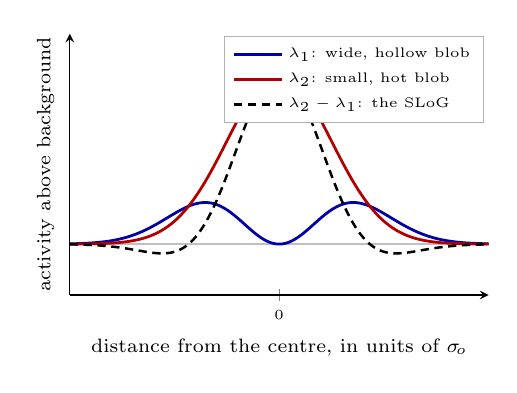
\begin{tikzpicture}
\begin{axis}[
  width=6.9cm, height=4.9cm,
  xmin=-4, xmax=4, ymin=-0.30, ymax=1.24,
  xlabel={distance from the centre, in units of $\sigma_{\!o}$}, ylabel={activity above background},
  ytick=\empty, xtick={0}, xticklabels={0},
  axis lines=left, enlargelimits=false,
  legend style={at={(0.99,0.99)},anchor=north east,font=\tiny,draw=black!30,
                legend cell align=left},
  tick label style={font=\tiny}, label style={font=\scriptsize},
]
  \addplot[black!25,line width=0.5pt,forget plot,domain=-4:4,samples=2] {0};
  \addplot[blue!65!black,line width=1pt,smooth,domain=-4:4,samples=250]
          {(x^2/3)*exp(-x^2/2)};
  \addlegendentry{$\lambda_1$: wide, hollow blob}
  \addplot[red!70!black,line width=1pt,smooth,domain=-4:4,samples=250]
          {exp(-x^2/2)};
  \addlegendentry{$\lambda_2$: small, hot blob}
  \addplot[black,densely dashed,line width=0.9pt,smooth,domain=-4:4,samples=250]
          {(1-x^2/3)*exp(-x^2/2)};
  \addlegendentry{$\lambda_2-\lambda_1$: the SLoG}
\end{axis}
\end{tikzpicture}
  \caption{The two hypotheses.}
\end{subfigure}
\\[1.6ex]
\begin{subfigure}[b]{0.95\textwidth}\centering
  \includegraphics{fig-slog2d.pdf}
  \caption{Transaxial cuts, at perfect resolution and after smoothing.}
\end{subfigure}
\caption{The detection task. \textbf{(a)} A cylinder of diameter $\Dcyl$ on the axis of a
detector of length $\Lpet$ and diameter $\Dpet$; shaded is the solid angle covered at $z$.
\textbf{(b, c)} The two hypotheses of Eq.~\eqref{eq:slog} --- a wide blob with a cold
interior and a small hot blob, of equal total activity --- and their difference, the SLoG,
as radial profiles and as transaxial cuts on a background $B$. The lesion contrast is
exaggerated for visibility. The bottom row of \textbf{(c)} repeats the three after smoothing
with a kernel of the SLoG size, on the same colour scales: the two hypotheses become hard to
tell apart and the difference peak falls by a factor of six.}
\label{fig:task}
\end{figure}

\paragraph{The result.}
Their expression can be rearranged, without approximation, into a product of four
independent factors (Appendix~\ref{sec:regroup}):
\begin{equation}
  \boxed{\;
  \mathrm{SNR}^{2}(z)=\;T\;\times
  \underbrace{\frac{\dot S^{2}\so^{3}}{16\pi\sqrt{\pi}\,\dot B}}
             _{\substack{\text{SLoG size}\\[1pt]\text{and contrast}}}
  \times
  \underbrace{\epsilon\,\eta_N(z)}
             _{\substack{\text{photon-pair}\\[1pt]\text{detection efficiency}}}
  \times
  \underbrace{r}
             _{\substack{\text{scanner resolution}\\[1pt]\text{vs.\ SLoG resolution}}} \;}
  \label{eq:grouped}
\end{equation}
Here $T$ is the total acquisition time; $\dot S$ and $\dot B$ are the count rates from the
SLoG and from the background, so the first factor is a property of the imaging task alone;
$\epsilon\,\eta_N(z)$ is the probability that a pair emitted at $z$ is recorded, discussed
below; and $r$ measures the resolutions of the scanner against the resolution $\so$ the task
demands. Writing $\sigma_y$ and $\sigma_z$ for the transverse and axial detector resolutions
and $\sigma_t$ for the TOF resolution expressed as a distance, $r$ depends on them only
through the three dimensionless \emph{resolution weights}
\begin{equation}
  w_t=\frac{\so^{2}}{\sigma_t^{2}+\so^{2}},\qquad
  w_y=\frac{\so^{2}}{\sigma_y^{2}+\so^{2}},\qquad
  w_z=\frac{\so^{2}}{\sigma_z^{2}+\so^{2}},
  \label{eq:weights}
\end{equation}
each running from $0$, when the system is far coarser than the task requires, to $1$, when
it is far finer. For a system with time of flight,
\begin{equation}
  \boxed{\;
  \rT(w_t,w_y,w_z)=\sqrt{w_t w_y w_z}\;
  \left(\tfrac{1}{2}\left(w_t+w_y+w_z\right)^{2}+w_t^{2}+w_y^{2}+w_z^{2}\right).\;}
  \label{eq:Fres}
\end{equation}
Letting $\sigma_t\to\infty$ here sends $w_t\to0$ and hence $\rT\to0$, which cannot be right:
a non-time-of-flight scanner is not blind. The reason is that Eq.~\eqref{eq:snr} assumes the
TOF kernel narrow compared with the object, so that limit lies outside its range of
validity. Nuyts et al.\ also give the expression that avoids the assumption, and taking
$\sigma_t\to\infty$ in \emph{it} leaves
\begin{equation}
  \boxed{\;
  \rN(w_y,w_z)=\frac{2\sqrt{\pi}\,\so}{\Dcyl}\,
  \sqrt{w_y w_z}\;\left(\tfrac{1}{2}\left(w_y+w_z\right)^{2}+w_y^{2}+w_z^{2}\right)\;}
  \label{eq:FnoTOF}
\end{equation}
as the factor $r$ for a scanner without time of flight (Appendix~\ref{sec:regroup}). Since
$\rT$ increases monotonically in each weight it is bounded, $0<\rT\le r_{\max}=\tfrac{15}{2}$,
attained when all three resolutions are far finer than the task demands; the ratio
$r/r_{\max}$ is therefore a natural figure of merit, collapsing four resolutions into one
number between $0$ and $1$.

Of the four factors, only $\epsilon\,\eta_N(z)$ depends on the scanner geometry, on the
object and on how the scan is organised, and only it depends on $z$. The rest of this
section says what it is; Sections~\ref{sec:recipe}--\ref{sec:beds} say how to evaluate it.

\paragraph{The two parts of the sensitivity factor.}
The fraction of emitted pairs that the system records lumps together the solid angle
subtended by the detector, the attenuation along the lines of response, and the probability
that a pair reaching the crystals is actually registered. The first two are geometry; the
third is not, and has to be measured. For a single bed position we therefore write
\begin{equation}
  \eta_{\mathrm{tot}}(z)=\epsilon\,\eta(z),
  \label{eq:split}
\end{equation}
with $\epsilon$ the \emph{average detector-pair efficiency} --- set by crystal material and
thickness, energy resolution and energy window, and independent of $z$ --- and $\eta(z)$ the
\emph{geometric sensitivity profile}, the fraction of $4\pi$ covered at axial position $z$,
reduced by the attenuation of the object. Section~\ref{sec:recipe} obtains $\epsilon$ from a
reported NEMA sensitivity; Section~\ref{sec:profile} computes $\eta(z)$.

\paragraph{Several overlapping bed positions.}
A clinical examination covers an axial range that is rarely equal to the length of the
scanner, so the scan is assembled from $N$ bed positions at axial offsets $z_1,\dots,z_N$ of
the object relative to the detector, generally overlapping. We assume throughout that the
\emph{total} time $T$ is divided equally, $T_{\mathrm{bed}}=T/N$, and that moving the bed
carries no time penalty; both are idealisations that favour large $N$, and we return to them
in Section~\ref{sec:beds}. Data recorded at different bed positions are statistically
independent, so the squared SNRs of the Hotelling observer add over them, and the entire
protocol enters through a single function, the time-weighted average of the single-bed
profile,
\begin{equation}
  \eta_N(z)=\frac{1}{N}\sum_{n=1}^{N}\eta(z-z_n).
  \label{eq:etaN}
\end{equation}
The product $\epsilon\,\eta_N(z)$ is then exactly what its name suggests: the probability
that a pair emitted at axial position $z$, at a uniformly random moment of the scan, is
recorded. For a single bed position it reduces to $\epsilon\,\eta(z)$. The factor $1/N$ is
the price of dividing a fixed total time between beds, and the sum is the gain from letting
several positions see the same point; scanner length, ring-difference limit, bed count and
overlap all act only through $\eta_N$, and choosing them is the subject of
Section~\ref{sec:beds}.

\paragraph{Evaluating this from published numbers.}
Resolutions are reported as full widths at half maximum, $F_i=\sqrt{8\ln2}\,\sigma_i$, and
almost no conversion is needed. The weights are ratios of two quantities of the same kind,
so the factors of $\sqrt{8\ln2}$ cancel and reported FWHM may be substituted directly,
\begin{equation}
  w_i=\frac{\so^{2}}{\sigma_i^{2}+\so^{2}}=\frac{\Fo^{2}}{F_i^{2}+\Fo^{2}},
  \qquad i=t,y,z .
  \label{eq:wFWHM}
\end{equation}
The only places $\so$ appears outside a ratio are the prefactor of Eq.~\eqref{eq:grouped},
where $\so^{3}=\Fo^{3}/\kf$, and Eq.~\eqref{eq:FnoTOF}, where
$2\sqrt{\pi}\,\so/\Dcyl=\Fo/(0.664\,\Dcyl)$. The timing resolution is published as a
coincidence time resolution in picoseconds; as a length,
$\Ft=\tfrac{c}{2}\,\mathrm{CTR}=0.15\,\mathrm{mm/ps}\times\mathrm{CTR}$, so
$200\,\mathrm{ps}$ becomes $30\,\mathrm{mm}$. Table~\ref{tab:eps} lists $\Ft$, $\Fy$ and
$\Fz$ for current systems in exactly this form.

The remainder of this paper is concerned with the detection-efficiency factor: how to obtain
$\epsilon$ from a reported NEMA sensitivity, and how to compute the single-bed profile
$\eta(z)$ from which $\eta_N$ is assembled.

\section{Computing the detector-pair efficiency}
\label{sec:recipe}

A cylindrical PET system does not detect every annihilation pair produced inside it. Two
quite different things reduce the count rate: \emph{geometry}, because most emission
directions miss the detector altogether, and \emph{detection physics}, because a photon that
does reach a crystal may not be recorded --- finite stopping power, acceptance energy window, gaps
between blocks, readout losses. Only the first can be computed from the dimensions of the
scanner; the second has to be measured. This section gives everything needed to obtain
$\epsilon$ for a given system. Appendix~\ref{sec:derivation} gives the derivation,
Section~\ref{sec:profile} computes the geometric profile $\eta(z)$,
and Section~\ref{sec:beds} optimises the bed positions.

\paragraph{Inputs.} Four numbers, all available from the specification sheet and the NEMA
NU~2 performance report:
\begin{itemize}\setlength{\itemsep}{1pt}
  \item $\Lpet$, the axial length of the detector;
  \item $\Dpet$, its diameter (the ring diameter), with $R=\Dpet/2$;
  \item $\Lmrd$, the maximum ring difference expressed as an axial length, i.e.\ the largest
        axial separation of the two ends of an accepted line of response. A ring difference
        is a count of rings; it becomes a length on multiplying by the axial ring pitch,
        $\Lpet$ divided by the number of crystal rings. Set
        $\Lmrd\ge\Lpet$ if no limit is applied;
  \item $\Snema$, the reported NEMA sensitivity in $\mathrm{cps/kBq}$, measured with a line
        source of length $\Lsrc=700\,\mathrm{mm}$ centred on the axis.
\end{itemize}
Axial positions $z$ are measured from the centre of the axial field of view, so the detector
occupies $-\Lpet/2\le z\le\Lpet/2$ and the line source $-\Lsrc/2\le z\le\Lsrc/2$
(Figure~\ref{fig:geom}).

\paragraph{Result.} Write $\Sid$ for the fraction of the emitted pairs that an otherwise
perfect scanner of this geometry would record from that line source. Everything
non-geometric is then collected into one number, the average detector-pair efficiency
\begin{equation}
  \boxed{\;\epsilon=\frac{\Snema}{1000\,\Sid}\;}
  \qquad (\Snema \text{ in } \mathrm{cps/kBq},\ \Sid \text{ dimensionless}),
  \label{eq:eps}
\end{equation}
the factor $1000$ being the only unit conversion involved. With the abbreviations
\begin{equation}
  h(x)=\sqrt{x^{2}+\Dpet^{2}},\qquad
  p_{\mathrm{MRD}}=\frac{\Lmrd}{h(\Lmrd)},\qquad
  \Lex=\big(\Lpet-\Lsrc\big)_+,
  \label{eq:hp}
\end{equation}
with $(x)_+=\max(x,0)$, so that $\Lex$ is the length of detector not covered by the source,
the geometric factor is given in closed form by
\begin{equation}
  \boxed{\;
  \Sid=
  \begin{dcases}
    \frac{h(\Lpet)-h(\Lex)}{\Lsrc}
      & \text{if } \Lmrd\ge \Lpet, \\[4pt]
    \frac{h(\Lmrd)-h(\Lex)}{\Lsrc}+\frac{\Lpet-\Lmrd}{\Lsrc}\,p_{\mathrm{MRD}}
      & \text{if } \Lex\le\Lmrd\le \Lpet, \\[4pt]
    p_{\mathrm{MRD}} & \text{if } \Lmrd\le\Lex .
  \end{dcases}\;}
  \label{eq:summary}
\end{equation}
\marginpar{\marginnotefont Eq.~\eqref{eq:summary} is identical to the corresponding result
in the original document, which writes $A$, $L$ and $A_{\mathrm{MR}}$ for $\Lpet$, $\Lsrc$
and $\Lmrd$.}%
The three branches correspond to the ring-difference limit binding nowhere, in the middle of
the source only, and everywhere; they agree where they meet, so the expression is continuous
in $\Lmrd$. $\Sid$ is a pure number between $0$ and $1$, and $\epsilon$ is the probability
that a pair whose line of response is geometrically acceptable is actually recorded as a
coincidence. %Its square root is the corresponding single-photon efficiency.

%\paragraph{Where the three branches come from.}
%At axial position $z$ the acceptance of the scanner is governed by a single length, the
%axial half-reach
%\begin{equation}
%  d_1(z)=\min\!\left(\frac{\Lpet}{2}-\abs{z},\ \frac{\Lmrd}{2}\right)_{\!+} ,
%  \label{eq:d1}
%\end{equation}
%the smaller of what the ends of the detector allow and what the ring-difference limit
%allows, and $\Sid$ is the average over the source of
%$\cos\theta_1=d_1/\sqrt{d_1^{2}+R^{2}}$. Figure~\ref{fig:regimes} plots $d_1(z)$ over the length of the source. Without a cap
%the profile is the triangle $\Lpet/2-\abs{z}$ truncated by the ends of the source; a cap
%that cuts the triangle inside the source turns it into a trapezoid; a cap below the triangle
%everywhere flattens it into a rectangle. Sloped parts of the profile integrate to a
%difference of two $h$ values, flat parts to a constant times a length, and the three
%branches are exactly the three ways of combining those two contributions.

\begin{figure}[tbp]
\centering
\begin{subfigure}[t]{0.32\textwidth}\centering
  \regimecyl{9}{5}{99}\\[0.6ex]\branchpanel{9}{5}{99}
  \caption{$\Lmrd\ge \Lpet$. The geometry binds everywhere, the acceptance narrows steadily
  towards the ends of the source, and the profile is a \emph{triangle}.}
\end{subfigure}\hfill
\begin{subfigure}[t]{0.32\textwidth}\centering
  \regimecyl{9}{5}{3.2}\\[0.6ex]\branchpanel{9}{5}{3.2}
  \caption{$(\Lpet\!-\!\Lsrc)_+\!\le\!\Lmrd\!\le\!\Lpet$. The cap binds near the centre
  only, and the profile is a \emph{trapezoid}.}
\end{subfigure}\hfill
\begin{subfigure}[t]{0.32\textwidth}\centering
  \regimecyl{9}{5}{1.3}\\[0.6ex]\branchpanel{9}{5}{1.3}
  \caption{$\Lmrd\!\le\!(\Lpet\!-\!\Lsrc)_+$. The cap binds over the whole source, every
  point sees the same solid angle, and the profile is a \emph{rectangle}.}
\end{subfigure}
\caption{The three branches of Eq.~\eqref{eq:summary}, for one detector and one source
length ($\Lsrc<\Lpet$) at three maximum ring differences. \textbf{Top:} the accepted solid
angle at three points along the source. \textbf{Bottom:} the axial half-reach
$d_1(z)=\min(\Lpet/2-\abs{z},\,\Lmrd/2)$, with the geometric limit dashed diagonally and the
cap dashed horizontally; the shaded area is what Eq.~\eqref{eq:master} integrates. Both rows
share the horizontal scale.}
\label{fig:regimes}
\end{figure}

%Appendix~\ref{sec:derivation} carries this out and gives the algebra in full.
%
%\paragraph{Worked example.} A long-axial-field-of-view system with $\Lpet=1060\,\mathrm{mm}$
%and $\Dpet=820\,\mathrm{mm}$, operated without a ring-difference limit, reports
%$\Snema=175.3\,\mathrm{cps/kBq}$. Here $\Lpet-\Lsrc=360\,\mathrm{mm}$, so the first branch
%applies:
%\begin{equation*}
%  h(\Lpet)=\sqrt{1060^{2}+820^{2}}=1340.1\,\mathrm{mm},\qquad
%  h(360)=\sqrt{360^{2}+820^{2}}=895.5\,\mathrm{mm},
%\end{equation*}
%\begin{equation*}
%  \Sid=\frac{1340.1-895.5}{700}=0.6351,
%  \qquad
%  \epsilon=\frac{175.3}{1000\times0.6351}=0.276 ,
%\end{equation*}
%i.e.\ a single-photon efficiency of $\sqrt{\epsilon}=0.53$, which is a sensible figure for
%$20\,\mathrm{mm}$ of LSO.
%
%\paragraph{A caution on the ring difference.} The same system is normally operated with a
%maximum ring difference of $85$ rings, and in that mode reports
%$\Snema=82.6\,\mathrm{cps/kBq}$. A ring difference is a count of rings, not a length; it
%becomes one through the axial ring pitch. The $1060\,\mathrm{mm}$ field of view holds $320$
%crystal rings, a pitch of $3.31\,\mathrm{mm}$, so
%$\Lmrd=85\times3.31=282\,\mathrm{mm}$. Two independent checks confirm this: the axial
%acceptance angle it implies, $\arctan(282/820)=19^{\circ}$, matches the $18^{\circ}$ quoted
%for that mode, and the unrestricted mode gives
%$\arctan(1060/820)=52^{\circ}$, exactly the figure quoted for $\mathrm{MRD}\,322$. Since
%$282<360$ the third branch applies,
%$\Sid=p_{\mathrm{MRD}}=282/\sqrt{282^{2}+820^{2}}=0.325$, and
%$\epsilon=82.6/325=0.254$ --- consistent with the $0.276$ above, as it must be, since
%$\epsilon$ is a property of the detectors and not of the acquisition mode. Pairing the
%restricted-mode sensitivity with $\Lmrd\ge\Lpet$ instead would have given
%$82.6/635=0.130$, low by more than a factor of two. The reported sensitivity and the value
%of $\Lmrd$ must always refer to the same acquisition.

Table~\ref{tab:eps} applies the recipe to ten current configurations, spanning four
detector designs, three vendors and axial lengths from $20\,\mathrm{cm}$ to
$148\,\mathrm{cm}$. The efficiencies group by crystal rather than by scanner: the two
Siemens systems, all $20\,\mathrm{mm}$ LSO, give $\epsilon=0.28$ even though their axial
lengths differ by a factor of four; the two GE lutetium-based entries give $0.35$--$0.39$;
the two $30\,\mathrm{mm}$ BGO systems $0.49$ and $0.52$ despite a four-fold difference in
length; and the two United Imaging systems, built on the thinnest crystals at
$18.1\,\mathrm{mm}$ LYSO, give $0.19$ and $0.22$. 

%That the geometry can be divided out this cleanly, leaving a number that
%tracks the crystal and not the scanner, is the main evidence that Eq.~\eqref{eq:summary}
%is doing its job. The residual spread within a crystal family is a useful diagnostic in
%its own right: it collects the packing fraction, the gaps between blocks and rings, the
%energy window and the detector non-uniformity, none of which the geometric model knows
%about. The energy columns are given because the window and the photopeak resolution are
%what decide how much of the recorded rate is scattered, and hence how far a model that
%ignores scatter --- as this one does --- can be pushed. One entry
%deserves a caveat: the Omni~128 sensitivity is a vendor figure with no published NEMA
%evaluation behind it, and is quoted elsewhere as $385\,\mathrm{cps/kBq}$, which would give
%$\epsilon=0.50$ instead.

\begin{sidewaystable}
\centering\footnotesize
\setlength{\tabcolsep}{3.5pt}
\input{table.tex}
\caption{Detector-pair efficiencies of ten current PET configurations, ordered by vendor
and detector design. $\Sid$ follows from Eq.~\eqref{eq:summary} with
$\Lsrc=700\,\mathrm{mm}$ and $\epsilon$ from Eq.~\eqref{eq:eps}; $\Snema$ is the NEMA NU~2
sensitivity for the centred line source. All resolutions are full widths at half maximum,
ready to be used directly in Eq.~\eqref{eq:wFWHM}, and the last two columns give the
resolution factor $r$ for two SLoG sizes: $\rT$ of Eq.~\eqref{eq:Fres} for the
time-of-flight systems, $\rN$ of Eq.~\eqref{eq:FnoTOF} with $\Dcyl=300\,\mathrm{mm}$ for the
two BGO ones. Notes and sources below.}
\label{tab:eps}
\vspace{1.2ex}
\parbox{0.99\textheight}{\footnotesize \textbf{Notes to Table~\ref{tab:eps}.} $\Ft=\tfrac{c}{2}\,\mathrm{CTR}$; $\Delta E/E$ is the
FWHM of the $511\,\mathrm{keV}$ photopeak; $\Fy$ is the mean of the radial and tangential
NEMA point-source FWHM at $1\,\mathrm{cm}$ from the axis, reconstructed by filtered
backprojection. The Omni~128 has no published performance evaluation; the entries marked
$^{\ast}$ are the resolutions of the Omni Legend~32, which uses the same detector, and the
$r$ values in that row rest on that assumption. The Biograph Vision~600 and Vision.X are the
same detector before and after an electronics upgrade: only the CTR differs,$^{9}$ and the
remaining entries are those of the original, for which alone a peer-reviewed evaluation
exists. $\Dpet$ is the detector face-to-face distance; for the two United Imaging systems it
is unpublished and $788\,\mathrm{mm}$ is inferred from the $62^{\circ}$ maximum acceptance
angle quoted for the GS, consistent with the $786\,\mathrm{mm}$ of the uEXPLORER.
\emph{Sources:}
$^{1}$J.~van Sluis et al., J.\ Nucl.\ Med.\ \textbf{60} (2019) 1031, energy resolution,
window and ring diameter from J.~S.~Reddin et al., IEEE NSS/MIC (2018) 1;
$^{2}$G.~A.~Prenosil et al., J.\ Nucl.\ Med.\ \textbf{63} (2022) 476;
$^{3}$A.~Chicheportiche et al., EJNMMI Phys.\ \textbf{7} (2020) 4, resolution and energy
resolution from D.~F.~C.~Hsu et al., J.\ Nucl.\ Med.\ \textbf{58} (2017) 1511, ring
diameter from D.~Vandendriessche et al., EJNMMI Phys.\ \textbf{6} (2019) 8;
$^{4}$K.~G.~Zeimpekis et al., Eur.\ J.\ Nucl.\ Med.\ Mol.\ Imaging \textbf{49} (2022) 3023;
$^{5}$S.~Yamagishi et al., J.\ Nucl.\ Med.\ \textbf{64} (2023) 1990 (the energy resolution
is asserted in the discussion of that paper rather than measured in it);
$^{6}$GE HealthCare product information (no published NEMA evaluation);
$^{7}$G.~Li et al., J.\ Nucl.\ Med.\ \textbf{65} (2024) 652;
$^{8}$H.~Zhang et al., J.\ Nucl.\ Med.\ \textbf{65} (2024) 1974;
$^{9}$H.~Zaidi et al., J.\ Nucl.\ Med.\ \textbf{66} (2025) suppl.\ 1, 251754 (abstract).}
\end{sidewaystable}


\begin{figure}[tbp]
\centering
%% tikz-geometry.tex --- included by sensitivity_derivation.tex
%% Figure 1: side view of the detector cylinder with the accepted solid angle.
%% Requires: tikz, pgfplots (compat=1.18), arrows.meta.

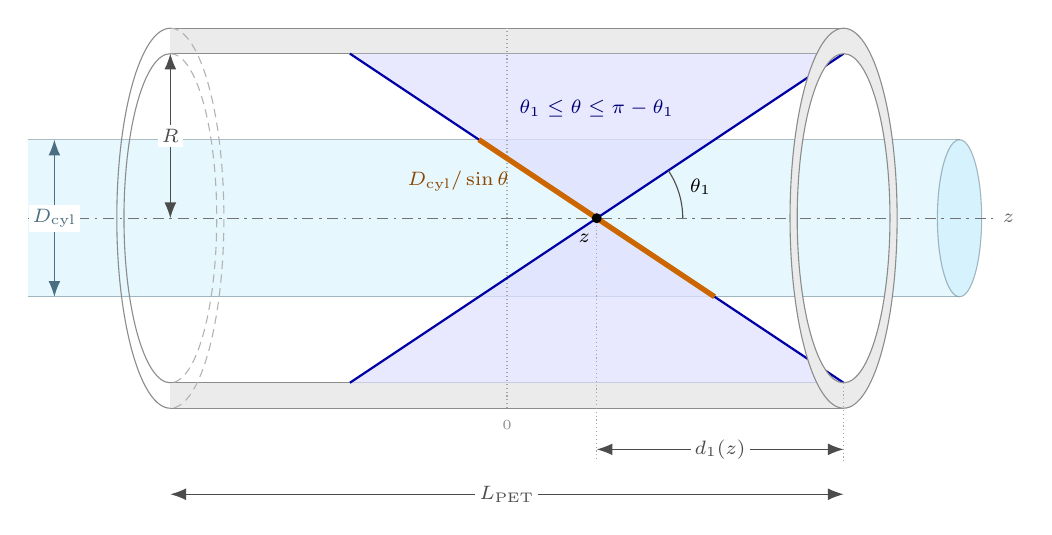
\begin{tikzpicture}[>={Latex[length=2mm]},scale=0.95]
  \pgfmathsetmacro{\A}{9}\pgfmathsetmacro{\R}{2.2}\pgfmathsetmacro{\zz}{1.2}
  \pgfmathsetmacro{\LL}{11}\pgfmathsetmacro{\Ah}{\A/2}
  \pgfmathsetmacro{\done}{\Ah-\zz}\pgfmathsetmacro{\zfar}{\zz-\done}
  \pgfmathsetmacro{\thone}{atan(\R/\done)}
  \pgfmathsetmacro{\ee}{0.62}\pgfmathsetmacro{\tw}{0.34}
  \pgfmathsetmacro{\eeo}{\ee*(\R+\tw)/\R}
  \pgfmathsetmacro{\rO}{1.05}\pgfmathsetmacro{\eO}{\ee*\rO/\R}
  % where the limiting LOR enters and leaves the attenuating cylinder
  \pgfmathsetmacro{\zin}{\zz-\done*\rO/\R}\pgfmathsetmacro{\zout}{\zz+\done*\rO/\R}

  % ---- detector cylinder, side view: walls and far rim -------------------
  \fill[black!8] (-\Ah,\R) rectangle (\Ah,{\R+\tw});
  \fill[black!8] (-\Ah,{-\R-\tw}) rectangle (\Ah,-\R);
  \draw[black!45] (-\Ah,\R) -- (\Ah,\R);   \draw[black!45] (-\Ah,{\R+\tw}) -- (\Ah,{\R+\tw});
  \draw[black!45] (-\Ah,-\R) -- (\Ah,-\R); \draw[black!45] (-\Ah,{-\R-\tw}) -- (\Ah,{-\R-\tw});
  % ---- uniform attenuating cylinder, longer than the scanner -------------
  \fill[cyan!10] (-\LL/2-0.9,-\rO) rectangle (\LL/2+0.55,\rO);
  \draw[cyan!40!black,opacity=0.45] (-\LL/2-0.9,\rO)  -- (\LL/2+0.55,\rO);
  \draw[cyan!40!black,opacity=0.45] (-\LL/2-0.9,-\rO) -- (\LL/2+0.55,-\rO);
  \fill[cyan!16] (\LL/2+0.55,0) ellipse ({\eO} and {\rO});
  \draw[cyan!40!black,opacity=0.45] (\LL/2+0.55,0) ellipse ({\eO} and {\rO});

  \draw[black!30,densely dashed] (-\Ah,\R)        arc ( 90:-90:{\ee} and {\R});
  \draw[black!30,densely dashed] (-\Ah,{\R+\tw})  arc ( 90:-90:{\eeo} and {\R+\tw});
  \draw[black!45] (-\Ah,\R)       arc ( 90:270:{\ee} and {\R});
  \draw[black!45] (-\Ah,{\R+\tw}) arc ( 90:270:{\eeo} and {\R+\tw});

  % ---- accepted solid angle: theta_1 <= theta <= pi - theta_1 ------------
  \fill[blue!12,opacity=0.75] (\zz,0) -- (\Ah,\R)  -- (\zfar,\R)  -- cycle;
  \fill[blue!12,opacity=0.75] (\zz,0) -- (\Ah,-\R) -- (\zfar,-\R) -- cycle;

  % ---- axis -------------------------------------------------------------
  \draw[dash pattern=on 4pt off 2pt on 1pt off 2pt,black!55]
        (-\LL/2-0.9,0) -- (\LL/2+1.0,0) node[right,font=\scriptsize,black!60] {$z$};
  \draw[black!35,thin,densely dotted] (0,{-\R-\tw}) -- (0,{\R+\tw});
  \node[font=\tiny,black!45,anchor=north] at (0,{-\R-\tw-0.04}) {$0$};

  % ---- limiting LORs ----------------------------------------------------
  \draw[blue!65!black,thick] (\zfar,-\R) -- (\Ah,\R);
  \draw[blue!65!black,thick] (\zfar,\R)  -- (\Ah,-\R);
  % the chord this LOR cuts through the attenuating cylinder
  \draw[orange!80!black,line width=1.9pt] (\zin,\rO) -- (\zout,-\rO);
  \node[orange!55!black,font=\scriptsize,anchor=east]
        at ({\zz-\done*0.50/\R-0.30},0.50) {$\Dcyl/\sin\theta$};

  % ---- near rim, drawn on top so the LORs terminate at the detector ------
  \fill[black!8,even odd rule] (\Ah,0) ellipse ({\eeo} and {\R+\tw})
                               (\Ah,0) ellipse ({\ee} and {\R});
  \draw[black!45] (\Ah,0) ellipse ({\eeo} and {\R+\tw});
  \draw[black!45] (\Ah,0) ellipse ({\ee} and {\R});

  % ---- source point, theta_1 --------------------------------------------
  \fill (\zz,0) circle (1.9pt);
  \node[font=\scriptsize,anchor=north east] at (\zz+0.04,-0.08) {$z$};
  \draw[black!70] (\zz+1.15,0) arc (0:\thone:1.15);
  \node[font=\scriptsize] at ({\zz+1.45*cos(\thone/2)},{1.45*sin(\thone/2)}) {$\theta_1$};
  % centroid of the upper shaded triangle sits at x = z, y = 2R/3
  \node[font=\scriptsize,blue!45!black] at (\zz,{0.667*\R})
        {$\theta_1\le\theta\le\pi-\theta_1$};

  % ---- dimensions -------------------------------------------------------
  \draw[<->,black!70] (-\Ah,0) -- (-\Ah,\R)
        node[midway,fill=white,inner sep=1.5pt,font=\scriptsize] {$R$};
  \draw[<->,cyan!45!black] (-\LL/2-0.55,-\rO) -- (-\LL/2-0.55,\rO)
        node[midway,fill=white,inner sep=1.5pt,font=\scriptsize] {$\Dcyl$};
  \draw[black!35,thin,densely dotted] (\zz,-0.1)  -- (\zz,{-\R-\tw-0.70});
  \draw[black!35,thin,densely dotted] (\Ah,{-\R}) -- (\Ah,{-\R-\tw-0.70});
  \draw[<->,black!70] (\zz,{-\R-\tw-0.55}) -- (\Ah,{-\R-\tw-0.55})
        node[midway,fill=white,inner sep=1.5pt,font=\scriptsize] {$d_1(z)$};
  \draw[<->,black!70] (-\Ah,{-\R-\tw-1.15}) -- (\Ah,{-\R-\tw-1.15})
        node[midway,fill=white,inner sep=1.5pt,font=\scriptsize] {$\Lpet$};
\end{tikzpicture}

\caption{Side view of the detector, of radius $R$ and axial length $\Lpet$, with the
attenuating object of diameter $\Dcyl$ in blue. Every LOR from a point on the axis is
symmetric about that point and meets the detector at $z\pm\delta$ with
$\delta=R\abs{\cot\theta}$; the blue lines are the two limiting accepted LORs, grazing the
near end, and the shaded wedge is the accepted solid angle
$\theta_1\le\theta\le\pi-\theta_1$. The orange segment is the chord $\Dcyl/\sin\theta$ that
enters the survival factor of Eq.~\eqref{eq:eta}.}
\label{fig:geom}
\end{figure}

\section{Axial sensitivity profile with attenuation}
\label{sec:profile}


This section computes the single-bed profile $\eta(z)$ from which the multi-bed profile
$\eta_N$ of Eq.~\eqref{eq:etaN} is assembled. The geometry is the one drawn in
Figure~\ref{fig:geom}, which carries the attenuating cylinder as well as the detector.

So far the only thing that could stop a pair was geometry: a direction was accepted if both
photons landed on the detector, and $\eta(z)$ was simply the accepted fraction of $4\pi$. If
the source sits inside a uniform cylinder of diameter $\Dcyl$ and linear attenuation
coefficient $\mu$, each accepted direction survives only with a probability that depends on
how much material the line of response crosses. For a point on the axis that chord is
$\Dcyl/\sin\theta$ (Figure~\ref{fig:geom}), and because the two photons \emph{together}
traverse the whole of it, the survival probability of the pair is
$\exp(-\mu\Dcyl/\sin\theta)$ --- the same wherever along the chord the annihilation
occurred.

The profile is that survival probability integrated over the accepted solid angle and
divided by $4\pi$. We work in spherical coordinates with the polar angle $\theta$ measured
from the $z$ axis and the azimuth $\phi$ about it, so that the solid-angle element is
$d\Omega=\sin\theta\,d\theta\,d\phi=-d(\cos\theta)\,d\phi$: solid angle is uniform in
$u=\cos\theta$. That is what makes the integral elementary --- the accepted directions are
$\abs{u}\le u_1(z)$, the integrand depends on $u$ alone, and nothing depends on $\phi$.
With $\sin\theta=\sqrt{1-u^{2}}$,
\begin{equation}
  \eta(z)=\frac{1}{4\pi}\int_0^{2\pi}\!\!d\phi\int_{-u_1(z)}^{u_1(z)}\!\!
          e^{-\mu \Dcyl/\sqrt{1-u^{2}}}\,du
        = \int_{0}^{u_1(z)} e^{-\mu \Dcyl/\sqrt{1-u^{2}}}\,du .
  \label{eq:eta}
\end{equation}

%Substituting $u=\sin\varphi$ gives the equivalent obliquity form
%$\int_0^{\beta(z)}\cos\varphi\,e^{-\mu \Dcyl/\cos\varphi}\,d\varphi$ with $\tan\beta=d_1/R$,
%and setting $\Dcyl=0$ recovers $\eta(z)=u_1(z)=\cos\theta_1(z)$, so Eq.~\eqref{eq:eta}
%contains the purely geometric profile as a special case. Both identities were checked
%numerically to machine precision.

%Two practical remarks. First, the exponential depends on $u$ and must therefore stay
%\emph{inside} the integral: Eq.~\eqref{eq:eta} has no closed form and is evaluated
%numerically. Pulling the attenuation out as $e^{-\mu \Dcyl}u_1$ is not permissible --- for
%$\mu \Dcyl=1.92$ (a $20\,\mathrm{cm}$ water cylinder) and $\theta_1=38^\circ$ it
%overestimates $\eta$ by $1.5\,\%$, and the error grows with both the acceptance and
%$\mu \Dcyl$. Second, the chord expression assumes the LOR leaves the phantom through its
%curved surface rather than through a flat end. That requires
%$\abs{z}+(\Dcyl/2R)\,d_1(z)\le \Lpet/2$, which reduces to $\abs{z}\le \Lpet/2$ whenever
%$\Dcyl<\Dpet$, and is therefore satisfied automatically as long as the attenuating cylinder
%is at least as long as the scanner.

Figure~\ref{fig:profile} shows $\eta(z)$ for four scanner lengths and three cylinder
diameters, one panel per diameter. Two features are worth noting, both of which follow
from Eq.~\eqref{eq:eta}. Note that the vertical scales differ by more than an order of
magnitude between the panels, and that the $\Dcyl=0$ curves are the purely geometric
profile $u_1(z)$. Attenuation does not simply scale the profile down, it also
\emph{flattens} it and slightly erodes the geometrical advantage of long scanners: the
centre of the field of view is where the most oblique directions are accepted, and those are
exactly the ones that cross the most material, $\Dcyl/\sqrt{1-u^{2}}$, whereas near the ends
only near-transaxial directions get through and the chord is close to $\Dcyl$.

%The centre
%of the field of view is where the most oblique LORs are accepted, and those are exactly the
%ones that cross the most material, $\Dcyl/\sqrt{1-u^{2}}$; near the ends only near-transaxial
%directions are accepted and the chord is close to $\Dcyl$. For $\Lpet=100\,\mathrm{cm}$ the
%profile value at $\abs{z}=45\,\mathrm{cm}$ relative to the peak therefore rises from $0.17$
%at $\Dcyl=0$ to $0.22$ at $20\,\mathrm{cm}$ and $0.24$ at $30\,\mathrm{cm}$.

%For the same reason, attenuation erodes the advantage of a long scanner. The ratio of the
%peak values for $\Lpet=100$ and $30\,\mathrm{cm}$ falls from $2.14$ at $\Dcyl=0$ to $1.73$
%at $20\,\mathrm{cm}$ and $1.59$ at $30\,\mathrm{cm}$: the extra length buys oblique
%directions, and in an attenuating object those are worth progressively less.

\begin{figure}[tbp]
\centering
\input{fig-profile.pgf}
\caption{Axial profile $\eta(z)$ of Eq.~\eqref{eq:eta}, one panel per object diameter;
colour is the axial length of the scanner, darker for longer, and each curve ends where
its detector does. Note
the different vertical scales; $\Dcyl=0$ gives the purely geometric profile $u_1(z)$. All
curves use $\Dpet=74\,\mathrm{cm}$, no ring-difference limit and
$\mu=0.0096\,\mathrm{mm^{-1}}$ (water at $511\,\mathrm{keV}$).}
\label{fig:profile}
\end{figure}

\section{Optimising the acquisition protocol}
\label{sec:beds}

A clinical examination has to cover an axial range $S$ that is rarely equal to the length of
the scanner, so the scan is assembled from $N$ bed positions sharing the total time $T$. We
judge a protocol by the \emph{worst} detectability anywhere in the range --- an examination
is only as good as its least-covered plane --- and ask for the arrangement that maximises it.

Of all the factors in Eq.~\eqref{eq:grouped}, only $\eta_N$ depends on how the scan is
organised. The acquisition time $T$, the SLoG factor, the detector-pair efficiency
$\epsilon$ and the resolution factor $r$ are constants with respect to $z$ and to the
protocol, so
\begin{equation}
  \max_{\text{protocol}}\ \min_{\abs{z}\le S/2}\mathrm{SNR}^{2}(z)
  \;=\;K\cdot\max_{\text{protocol}}\ \min_{\abs{z}\le S/2}\eta_N(z),
  \qquad K>0 \ \text{fixed}.
  \label{eq:decouple}
\end{equation}
Choosing the bed positions is therefore a pure geometry problem: the answer is independent
of the SLoG, of the scan time, of the crystal and of the spatial and TOF resolutions, and
depends only on the single-bed profile $\eta(z)$ and on $S$.\footnote{This relies on $r$
being independent of $z$, which holds because we evaluate on the axis. If the spatial
resolution were allowed to degrade with obliquity or with radial position, $r$ would become
a function of $z$ and the two problems would couple.}

With the time per bed fixed at $T_{\mathrm{bed}}=T/N$ and a constant spacing $d$ between
neighbouring beds --- a single constant overlap $1-d/\Lpet$ is what scanners normally let
one set --- the protocol has two free parameters, $N$ and $d$, and the problem is
\begin{equation}
  \boxed{\;M(S)=\max_{N,\,d}\;\min_{\abs{z}\le S/2}\;
       \frac{1}{N}\sum_{n=1}^{N}\eta\!\left(z-\Big(n-\tfrac{N+1}{2}\Big)d\right).\;}
  \label{eq:maxmin}
\end{equation}

\paragraph{What the problem looks like.}
Figure~\ref{fig:ripple} shows it for a $100\,\mathrm{cm}$ detector asked to cover
$150\,\mathrm{cm}$ in a $20\,\mathrm{cm}$ cylinder. A single bed position fails outright:
the range extends $25\,\mathrm{cm}$ beyond each end of the detector, where $\eta$ vanishes,
so the minimum is zero. From $N=2$ on the range is covered, but the achievable minimum is
not a smooth function of $N$. Superposing shifted copies of $\eta$ does not give a flat
profile, it gives a rippled one, and the minimum is set by the deepest trough; how deep the
troughs are depends on how the copies interleave. Here $N=5$ tiles the range almost
smoothly and wins, while $N=4$ --- whose optimal spacing is exactly $\Lpet/2$, the
conventional $50\,\%$ overlap --- places its troughs worst and is $22\,\%$ below its
immediate neighbours. Beyond $N\simeq5$ the curve flattens out: further bed positions tile
the range a little more evenly but add nothing, which is remark (ii) below in visual form.

\paragraph{Solving it.}
Equation~\eqref{eq:maxmin} has no closed-form solution for a realistic $\eta$, and the inner
minimum makes it non-smooth in $d$, so we solve it numerically. The recipe is short enough
to state in full. Tabulate $\eta(z)$ once on a fine grid over $[-\Lpet/2,\Lpet/2]$ by
evaluating Eq.~\eqref{eq:eta}, and interpolate. For a given $N$, sweep the spacing $d$ over
$[0,\Lpet]$ on a coarse grid, evaluating for each $d$ the minimum of the superposition over
a grid of $z$ in $[-S/2,S/2]$; keep the best $d$ and repeat on a refined interval around it
a few times. Then loop over $N$ from $1$ upwards and keep the best. The whole calculation
takes a second and is done by \texttt{make\_figures.py}; refining the search for $d$ by a
further factor of eight changes the computed minima by one part in $10^{9}$.

Three remarks complete the picture.

\emph{(i) When is one bed enough?} Since the minimum is bounded by the average of any two
samples, evaluating at $z=\pm S/2$ and using the symmetry of $\eta$ shows that moving beds
outwards can only help once $\eta(0)/2>\eta(S/2)$, i.e.\ once the range edge lies beyond the
half-maximum of the profile. Hence
\begin{equation}
  \boxed{\;\text{a single bed position is optimal as long as } S\le\mathrm{FWHM}\big(\eta\big).\;}
  \label{eq:fwhmrule}
\end{equation}
Numerically this threshold coincides with the FWHM to within a few per cent for every
geometry we tested. It is more permissive than it sounds: the FWHM is $75\,\mathrm{cm}$ for
a $100\,\mathrm{cm}$ detector and $124\,\mathrm{cm}$ for a $150\,\mathrm{cm}$ one, so a
$1\,\mathrm{m}$ oncological scan is best acquired in a \emph{single} bed position on a
total-body system, and splitting it would only waste time.

\emph{(ii) Overlapping beds cannot create sensitivity.} Shifting and averaging conserves
area, $\int\eta_N=\int\eta$ for every $N$ and every arrangement, because the factor $1/N$
cancels the $N$ copies exactly. With $T_{\mathrm{bed}}=T/N$ and no transport overhead, extra
bed positions only \emph{redistribute} sensitivity --- they flatten the profile, which is
the point, but they never add to it. In particular the minimum can never exceed the mean,
\begin{equation}
  M(S)\;\le\;M_{\max}(S)=\frac{1}{S}\int_{-S/2}^{S/2}\eta(z)\,dz ,
  \label{eq:ceiling}
\end{equation}
and $M/M_{\max}$ measures how flat a protocol manages to make the profile.

\emph{(iii) The bed count is only determined to within a tolerance.} Where the curves for
different $N$ cross, the best and second-best differ by less than about one per cent, which
carries no clinical meaning, and a plain maximisation then jumps around: at $S=145$, $150$
and $155\,\mathrm{cm}$ the winner would be $N=2$, $5$ and $3$ respectively. We therefore
report the \emph{smallest} $N$ that comes within $3\,\%$ of the best (shaded band in
Figure~\ref{fig:ripple}). That makes the reported bed count monotone in $S$, costs at most
$3\,\%$ of the achievable minimum, and is the sensible choice in practice since each extra
bed costs transport time that this model ignores. The quantity to trust is $M(S)$, which is
smooth.

\paragraph{Results.}
Figure~\ref{fig:beds} gives the optimised protocol as a function of the axial range, for
detectors of $30$, $100$ and $150\,\mathrm{cm}$ axial length in cylinders of $20$ and
$30\,\mathrm{cm}$ diameter; the dashed verticals mark three clinically representative
ranges, $20\,\mathrm{cm}$ (single organ or brain), $100\,\mathrm{cm}$ (oncological FDG scan
of the torso) and $180\,\mathrm{cm}$ (total body). Three observations. The single-bed
plateaus in the third row match the FWHM rule in every case; the FWHM of $\eta$ is
$16$--$17\,\mathrm{cm}$ for the $30\,\mathrm{cm}$ detector, $75$--$77\,\mathrm{cm}$ for the
$100\,\mathrm{cm}$ one and $124$--$127\,\mathrm{cm}$ for the $150\,\mathrm{cm}$ one. The
optimal overlap, in the bottom row, sawtooths between about $15$ and $48\,\%$ --- falling
as the range grows at fixed $N$, jumping back up each time $N$ steps --- and stays below the
$50\,\%$ often adopted by default essentially everywhere. And, conveniently, the optimal protocol
barely responds to the size of the patient: the two columns are nearly identical, even
though the achievable detectability differs between them by a factor of about three.\footnote{The only case with an analytic answer is a short scanner
with negligible attenuation, whose profile is close to the triangle
$\eta(z)=\eta(0)(1-\abs{z}/a)_+$ with $a=\Lpet/2$. Below $S=a$ every $N$ gives
\emph{precisely} the same minimum $\eta(0)(1-S/2a)$, since on a linear flank whatever a bed
gains at one edge it loses at the other; above it the optimum is $N=1+\lceil S/a\rceil$ beds
at spacing $d=S/(N-1)$, and when $S$ is an exact multiple of $a$ the shifted triangles tile
without ripple and give $M=\eta(0)/(1+S/a)$. That is the $1/(1+2S/\Lpet)$ falloff the
realistic profiles follow approximately in Figure~\ref{fig:beds}.}

\begin{figure}[tbp]
\centering
\input{fig-ripple.pgf}
\caption{The bed-optimisation problem of Eq.~\eqref{eq:maxmin}, for
$\Lpet=100\,\mathrm{cm}$, $\Dcyl=20\,\mathrm{cm}$ and $S=150\,\mathrm{cm}$. \textbf{Left:}
the achievable minimum of $\eta_N$ against $N$, each $N$ at its own optimal spacing; the
shaded band is within $3\,\%$ of the best and the circled point is the smallest $N$ inside
it. \textbf{Right:} the corresponding profiles $\eta_N(z)$, with each minimum marked.}
\label{fig:ripple}
\end{figure}

\begin{figure}[tbp]
\centering
\input{fig-beds.pgf}
\caption{The optimised protocol against the axial range $S$, for three detector lengths
(colour, darker for longer) and two object diameters (columns). \textbf{Rows:} the achievable minimum $M(S)$ of
Eq.~\eqref{eq:maxmin} on a linear and a logarithmic scale, the optimal bed count, and the
optimal overlap $1-d/\Lpet$, blank wherever one bed suffices. The dotted line marks the
conventional $50\,\%$ overlap; dashed verticals the three scan lengths quoted in the text.
Bed counts are the smallest $N$ within $3\,\%$ of the best. All curves use
$\Dpet=74\,\mathrm{cm}$ and no ring-difference limit.}
\label{fig:beds}
\end{figure}

\section{Comparing systems on the task}
\label{sec:compare}

Everything needed is now in place, so we close by evaluating Eq.~\eqref{eq:grouped} for a
set of realistic systems. Ten configurations are built from four detector designs, labelled \textbf{A}--\textbf{D}
and drawn from the four crystal families of Table~\ref{tab:eps}. Each carries its own
detector-pair efficiency, its own resolutions and its own bore, and is taken at one or two
axial lengths:
\begin{itemize}\setlength{\itemsep}{2pt}
  \item \textbf{A}, $3.2\times3.2\times20\,\mathrm{mm}$ LSO with $\epsilon=0.28$, a
        coincidence time resolution of $213\,\mathrm{ps}$ ($\Ft=32\,\mathrm{mm}$),
        $\Fy=\Fz=3.6\,\mathrm{mm}$ and $\Dpet=82\,\mathrm{cm}$, at $\Lpet=26$ and
        $106\,\mathrm{cm}$, the latter also with $\Lmrd=28\,\mathrm{cm}$;
  \item \textbf{B}, $3.95\times5.3\times25\,\mathrm{mm}$ LYSO with $\epsilon=0.36$,
        $380\,\mathrm{ps}$ ($\Ft=57\,\mathrm{mm}$), $\Fy=4.2$, $\Fz=4.5\,\mathrm{mm}$ and
        $\Dpet=74\,\mathrm{cm}$, at $\Lpet=20$ and $30\,\mathrm{cm}$;
  \item \textbf{C}, $4.1\times4.1\times30\,\mathrm{mm}$ BGO with $\epsilon=0.50$ and no time
        of flight, $\Fy=4.3$, $\Fz=4.4\,\mathrm{mm}$ and $\Dpet=73\,\mathrm{cm}$, at
        $\Lpet=32$ and $128\,\mathrm{cm}$;
  \item \textbf{D}, $2.76\times2.76\times18.1\,\mathrm{mm}$ LYSO with $\epsilon=0.20$,
        $187\,\mathrm{ps}$ ($\Ft=28\,\mathrm{mm}$), $\Fy=2.9$, $\Fz=2.8\,\mathrm{mm}$ and
        $\Dpet=79\,\mathrm{cm}$, at $\Lpet=35$, $70$ and $148\,\mathrm{cm}$.
\end{itemize}
Each is asked to cover an axial range from $5$ to $200\,\mathrm{cm}$ with its own optimised
protocol, in a $20$ and in a $30\,\mathrm{cm}$ cylinder, for a high-resolution task
($\Fo=5\,\mathrm{mm}$) and a low-resolution one ($\Fo=10\,\mathrm{mm}$).
Figure~\ref{fig:scen} is the result. Since $T$, $\dot S$ and $\dot B$ are common to all
systems, we plot $\mathrm{SNR}^2_{\min}$ in units of $T\dot S^{2}/(16\pi\sqrt{\pi}\dot B)$,
so the curves are $\so^{3}\epsilon\,\min_z\eta_N(z)\,r$ and only ratios within a panel carry
meaning.



Five things stand out.

\emph{All three scanner factors enter multiplicatively, so none can be neglected.}
$\mathrm{SNR}^{2}$ is linear in $\epsilon$, so detector \textbf{C}'s $0.50$ against
\textbf{D}'s $0.20$ is worth a genuine factor $2.5$. But \textbf{C} buys that thick crystal
at the price of coarse detectors and no time of flight, giving $r=0.028$ against $0.309$ at
$\Fo=5\,\mathrm{mm}$; the factor $11$ in $r$ wins, and the $148\,\mathrm{cm}$ \textbf{D}
system beats the $128\,\mathrm{cm}$ \textbf{C} one six-fold over a $1\,\mathrm{m}$ range.
The lesson is not that $\epsilon$ matters little, but that in these designs a high $\epsilon$
is bought with a low $r$.

\emph{Length pays, but less than a solid-angle argument suggests.} Going from $35$ to
$148\,\mathrm{cm}$, a factor $4.2$, buys a factor $8.0$ over a $1\,\mathrm{m}$ range ---
roughly $\Lpet^{1.5}$, not the $\Lpet^{2}$ that counting solid angle at a point would
suggest. The extra length buys oblique lines of response, and those are exactly the ones
attenuation removes: the same gain falls to $7.8$ in a $30\,\mathrm{cm}$ cylinder.

\emph{A ring-difference limit costs less than one might fear.} Restricting the
$106\,\mathrm{cm}$ system to $\Lmrd=28\,\mathrm{cm}$ costs a factor $1.9$ over a
$20\,\mathrm{cm}$ range in a $20\,\mathrm{cm}$ cylinder, but only $1.4$ over a
$180\,\mathrm{cm}$ range in a $30\,\mathrm{cm}$ one: attenuation has already suppressed most
of what the limit discards, and over a long range the bed arrangement flattens the profile
in any case.

\emph{Naming the task is not a formality: it changes the ranking.} At $\Fo=10\,\mathrm{mm}$
over a $20\,\mathrm{cm}$ range the $106\,\mathrm{cm}$ \textbf{A} and $148\,\mathrm{cm}$
\textbf{D} systems are indistinguishable, $1.62$ against $1.61$; sharpening the task to
$\Fo=5\,\mathrm{mm}$ puts the latter $31\,\%$ ahead. Further down the list the reversal is
outright: the $128\,\mathrm{cm}$ \textbf{C} system beats the $35\,\mathrm{cm}$ \textbf{D}
one by $30\,\%$ at $\Fo=10\,\mathrm{mm}$ and loses to it by $26\,\%$ at
$\Fo=5\,\mathrm{mm}$. This is the Muehllehner effect of Nuyts et al.\ in a system
comparison: as the demanded resolution approaches the detector resolution, $r$ rewards fine
detectors steeply, and two systems can trade places purely because the lesion of interest
got smaller.

\emph{A larger patient penalises a non-TOF system twice.} Going from a $20$ to a
$30\,\mathrm{cm}$ cylinder costs the time-of-flight systems a factor of about $2.8$ and the
non-time-of-flight ones about $4.4$. Everyone loses to attenuation; a system without TOF
loses again because the chord that plays the role of its TOF kernel in
Eq.~\eqref{eq:FnoTOF} grows with the object.

\begin{figure}[tbp]
\centering
\input{fig-scenarios.pgf}
\caption{Detectability of the SLoG for ten configurations, against the axial range $S$
each covers with its own optimised protocol. Colour and the letters \textbf{A}--\textbf{D}
identify the detector, line style the scanner: \emph{solid} for a long one
($>1\,\mathrm{m}$), \emph{dashed} and \emph{dotted} for short ones, \emph{dash-dotted} for
the $106\,\mathrm{cm}$ system restricted to $\Lmrd=28\,\mathrm{cm}$. Rows are the two SLoG
sizes crossed with the two object diameters. Each legend block ends with the resolution
factor $r$ of that detector at $\Fo=5$ and $10\,\mathrm{mm}$. The vertical axis is
$\so^{3}\epsilon\min_z\eta_N(z)\,r$ in units of $T\dot S^{2}/(16\pi\sqrt{\pi}\dot B)$, common
to all systems, so ratios within a panel are meaningful and the absolute scale is not.}
\label{fig:scen}
\end{figure}

%%%%%%%%%%%%%%%%%%%%%%%%%%%%%%%%%%%%%%%%%%%%%%%%%%%%%%%%%%%%%%%%%%%%%%%%%%%%%%%%
%%%%%%%%%%%%%%%%%%%%%%%%%%%%%%%%%%%%%%%%%%%%%%%%%%%%%%%%%%%%%%%%%%%%%%%%%%%%%%%%
%%%%%%%%%%%%%%%%%%%%%%%%%%%%%%%%%%%%%%%%%%%%%%%%%%%%%%%%%%%%%%%%%%%%%%%%%%%%%%%%

\clearpage

\appendix
\renewcommand{\theequation}{A.\arabic{equation}}\setcounter{equation}{0}
\renewcommand{\thefigure}{A.\arabic{figure}}\setcounter{figure}{0}

\section{Equivalence with the result of Nuyts et al.}
\label{sec:regroup}

Nuyts et al.\ (footnote~\ref{fn:nuyts}) give the squared signal-to-noise ratio of the
Hotelling observer for the SLoG task, for a Gaussian TOF kernel narrow compared with the
object, as
\begin{multline}
  \mathrm{SNR}^{2}=\frac{\eta_{\mathrm{tot}}}{16\pi\sqrt{\pi}}\,
  \frac{(S\so^{4})^{2}}{B}\,
  \frac{\so^{2}}{\sqrt{(\vt)(\vy)(\vz)}}\\[2pt]
  \times\left(\frac{1}{2}\left(\frac{1}{\vt}+\frac{1}{\vy}+\frac{1}{\vz}\right)^{\!2}
        +\frac{1}{(\vt)^{2}}+\frac{1}{(\vy)^{2}}+\frac{1}{(\vz)^{2}}\right).
  \label{eq:snr}
\end{multline}
The rearrangement used in Section~\ref{sec:aim} is elementary. With the weights of
Eq.~\eqref{eq:weights}, $w_i=\so^{2}/(\sigma_i^{2}+\so^{2})$, the two resolution-dependent
factors of Eq.~\eqref{eq:snr} are
\begin{equation}
  \frac{\so^{2}}{\sqrt{\textstyle\prod_i(\sigma_i^{2}+\so^{2})}}
     =\frac{\sqrt{w_t w_y w_z}}{\so},
  \qquad
  \frac{1}{2}\Big(\sum_i\frac{1}{\sigma_i^{2}+\so^{2}}\Big)^{\!2}
     +\sum_i\frac{1}{(\sigma_i^{2}+\so^{2})^{2}}
     =\frac{1}{\so^{4}}\left[\tfrac12\Big(\sum_i w_i\Big)^{\!2}+\sum_i w_i^{2}\right],
\end{equation}
so their product is $\rT/\so^{5}$ with $\rT$ as defined in Eq.~\eqref{eq:Fres}. Together
with $(S\so^{4})^{2}=S^{2}\so^{8}$ this collapses Eq.~\eqref{eq:snr} to
$\mathrm{SNR}^{2}=\eta_{\mathrm{tot}}S^{2}\so^{3}\rT/(16\pi\sqrt{\pi}B)$; substituting
$\eta_{\mathrm{tot}}=\epsilon\,\eta_N$ from Eqs.~\eqref{eq:split} and \eqref{eq:etaN} and
$S=\dot S T$, $B=\dot B T$ gives Eq.~\eqref{eq:grouped}. No approximation is involved: the
two forms are algebraically identical. As an independent check, Eq.~\eqref{eq:Fres}
reproduces the published resolution ratios obtained from Eq.~\eqref{eq:snr} --- improving
the detector resolution from $4.5$ to $1.5\,\mathrm{mm}$ FWHM raises $r$ by a factor $124$
for a $1.5\,\mathrm{mm}$ SLoG and by $3.15$ for a $6\,\mathrm{mm}$ SLoG, at a coincidence
time resolution of $214\,\mathrm{ps}$.

\paragraph{The non-TOF limit.}
Equation~\eqref{eq:snr} assumes the TOF kernel to be narrow compared with the object, so it
cannot be continued to $\sigma_t\to\infty$. Nuyts et al.\ also give the expression that
avoids the assumption, their Eq.~(53), which keeps the background profile $B(x)$ inside the
integral along the line of response and consists of three terms. As $\sigma_t\to\infty$ the
integral $\int G_1(x,\sigma_t')^2/[B(x)*G_1(x,\sigma_t)]\,dx$ tends to $1/(B\Dcyl)$,
independently of $\so$, so only the term in which both derivatives act on the transverse
factors survives; that term carries the function the authors obtain from their $\Phi$ by
dropping every factor and term involving the TOF variance. The result is
Eq.~\eqref{eq:FnoTOF}. Equivalently, a scanner without TOF behaves like one with a Gaussian
TOF kernel of standard deviation $\sigma_t^{\mathrm{eq}}=\Dcyl/(2\sqrt{\pi})$, i.e.\
$\Ft^{\mathrm{eq}}=0.664\,\Dcyl$ in FWHM --- the constant being Tomitani's. Two remarks are
worth recording. The length that fixes the equivalent kernel is the extent of the
\emph{background activity} along the line of response, not the length of the line of
response: empty space between object and detector carries no counts and hence no noise, so
the diameter of the scanner does not enter. And in practice $\Ft^{\mathrm{eq}}\gg\Fo$, so
$w_t$ is negligible in the additive bracket anyway and one may simply substitute
$\Ft=0.664\,\Dcyl$ into Eq.~\eqref{eq:Fres} and use a single expression for every scanner;
that shortcut agrees with Eq.~\eqref{eq:FnoTOF} to better than $0.2\,\%$. The closed form
was checked against a direct numerical evaluation of Eq.~(53) for cylinder diameters of
$10$, $20$ and $30\,\mathrm{cm}$, agreeing to eight significant figures
(\texttt{check\_nontof} in \texttt{make\_figures.py}).


\section{Derivation of the closed form}
\label{sec:derivation}

\subsection{The idea}

$\Sid$ is an average of a local quantity. At a single point of the source, the fraction of
the emitted pairs that the detector can intercept is the fraction of the full $4\pi$ that
the accepted directions occupy. Because the source lies on the axis and the two photons of
a pair leave back to back, every accepted line of response is symmetric about the emission
point, and the acceptance at $z$ is governed by one length --- the axial half-reach
\begin{equation}
  d_1(z)=\min\!\left(\frac{\Lpet}{2}-\abs{z},\ \frac{\Lmrd}{2}\right)_{\!+} ,
  \label{eq:d1app}
\end{equation}
the smaller of what the ends of the detector allow and what the ring-difference limit
allows, the positive part ensuring that points beyond the ends of the detector contribute
nothing. The covered fraction at that point turns out to be
\begin{equation}
  \frac{\Omega_{\mathrm{PS}}(z)}{4\pi}=\cos\theta_1(z)=\frac{d_1(z)}{\sqrt{d_1^2(z)+R^2}} ,
  \label{eq:frac}
\end{equation}
and $\Sid$ is simply the \emph{average of this fraction over the points of the line
source}:
\begin{equation}
  \Sid=\frac{1}{\Lsrc}\int_{-\Lsrc/2}^{\Lsrc/2}\cos\theta_1(z)\,dz .
  \label{eq:Sid}
\end{equation}
That is the whole content of the calculation; the rest of this section establishes
Eq.~\eqref{eq:frac} and evaluates the integral.

\subsection{Solid angle covered at a point on the axis}
\label{sec:omega}

Use spherical coordinates about the scanner axis: $\theta$ is the polar angle measured from
the $+z$ direction and $\phi$ the azimuth around the axis, so that the differential solid
angle takes its usual form
\begin{equation}
  d\Omega=\sin\theta\,d\theta\,d\phi=-\,d(\cos\theta)\,d\phi .
  \label{eq:dOmega}
\end{equation}
The second form is the useful one: solid angle is distributed \emph{uniformly} in
$u=\cos\theta$, so any calculation of a covered solid angle about the axis reduces to
measuring an interval in $u$. (An equally common choice is the obliquity
$\varphi=\pi/2-\theta$, measured from the transaxial plane rather than from the axis, for
which $u=\sin\varphi$ and $du=\cos\varphi\,d\varphi$. The factor $\cos\varphi$ that appears
in formulations based on the obliquity is nothing but this Jacobian.)

Because the source point lies on the axis, the two photons of a pair travel in exactly
opposite directions and the LOR is symmetric about that point: it meets the detector
cylinder at $z+\delta$ and $z-\delta$ with
\begin{equation}
  \delta=R\,\abs{\cot\theta}=R\,\frac{\abs{u}}{\sqrt{1-u^{2}}} .
  \label{eq:delta}
\end{equation}
A coincidence is recorded only if \emph{both} ends fall on the detector,
$z+\delta\le \Lpet/2$ and $z-\delta\ge-\Lpet/2$; if a maximum ring difference is applied,
the axial separation of the two ends is $2\delta$, giving the additional condition
$2\delta\le\Lmrd$. All three constraints act on the single quantity $\delta$, which is why
the acceptance is governed by the one length $d_1(z)$ of Eq.~\eqref{eq:d1app}: the condition
$\delta\le d_1$ is, through Eq.~\eqref{eq:delta}, the condition
\begin{equation}
  \abs{u}\le u_1(z)=\frac{d_1(z)}{\sqrt{d_1^2(z)+R^2}}=\cos\theta_1(z) .
  \label{eq:u1}
\end{equation}

It is worth noting that the two axial reaches, towards $+z$ and towards $-z$, cannot enter
separately: any expression in which they appear as two independent terms describes the
acceptance of \emph{single} photons, not of coincidences, and overestimates the result
everywhere except at $z=0$.

The covered solid angle now requires no integration worth the name,
\begin{equation}
  \Omega_{\mathrm{PS}}(z)=\int_0^{2\pi}\!\!d\phi\int_{-u_1}^{u_1}\!\!du = 4\pi\,u_1(z) ,
  \label{eq:omega}
\end{equation}
so the fraction of the pairs emitted at $z$ that produces a coincidence is
$\Omega_{\mathrm{PS}}(z)/4\pi=u_1(z)=\cos\theta_1(z)$, which is Eq.~\eqref{eq:frac}. For an
infinitely long detector $u_1\to1$ and the fraction tends to unity, as it must.

\subsection{Averaging along the line source}

A line source is a uniform superposition of point sources, each emitting independently, so
the count rates simply add and the total is the integral of $\Omega_{\mathrm{PS}}$ along the
source. Points outside the axial field of view have $d_1=0$ and contribute nothing, so with
$z_1=\min(\Lsrc/2,\Lpet/2)$ and using the symmetry about $z=0$,
\begin{equation}
  I_\Omega \;=\; \int_{-\Lsrc/2}^{\Lsrc/2}\!\!\Omega_{\mathrm{PS}}(z)\,dz
  \;=\;2\int_{0}^{z_1} 4\pi\,u_1(z)\,dz .
  \label{eq:Iomega}
\end{equation}
Dividing by $4\pi$ turns the integral into a fraction and dividing by $\Lsrc$ turns it into
a mean, which is Eq.~\eqref{eq:Sid}, $\Sid=I_\Omega/(4\pi \Lsrc)$.

\subsection{Evaluating the integral: the three branches}
\label{sec:equiv}

Substituting $s=\Lpet/2-z$, so that $d_1=\min(s,m)$ with $m=\Lmrd/2$, and noting that $s$
runs from $s_{\min}=\Lpet/2-z_1=(\Lpet-\Lsrc)_+/2$ up to $\Lpet/2$,
\begin{equation}
  \Sid=\frac{2}{\Lsrc}\int_{s_{\min}}^{\Lpet/2}
        \frac{\min(s,m)}{\sqrt{\min(s,m)^2+R^2}}\;ds ,
  \label{eq:master}
\end{equation}
with the antiderivative $\int s\,ds/\sqrt{s^{2}+R^{2}}=\sqrt{s^{2}+R^{2}}$.
Equation~\eqref{eq:master} is the complete result: the maximum ring difference enters only
through a $\min$ inside the integrand, and no case distinction is needed at this stage. The
cases appear only on evaluation, and throughout we use
$2\sqrt{x^{2}+R^{2}}=\sqrt{(2x)^{2}+\Dpet^{2}}$ together with the definitions
\eqref{eq:hp}.

\paragraph{(i) $m\ge \Lpet/2$, i.e.\ $\Lmrd\ge \Lpet$ (no effective cap).}
Then $\min(s,m)=s$ over the whole range and
\begin{equation}
  \Sid=\frac{2}{\Lsrc}\left[\sqrt{\Big(\tfrac{\Lpet}{2}\Big)^{2}+R^{2}}
       -\sqrt{\Big(\tfrac{(\Lpet-\Lsrc)_+}{2}\Big)^{2}+R^{2}}\right]
      =\frac{1}{\Lsrc}\Big[h(\Lpet)-h\big((\Lpet-\Lsrc)_+\big)\Big] ,
\end{equation}
the first branch of Eq.~\eqref{eq:summary}.

\paragraph{(ii) $s_{\min}\le m\le \Lpet/2$, i.e.\ $(\Lpet-\Lsrc)_+\le\Lmrd\le \Lpet$.}
Split the integral at $s=m$. On $[s_{\min},m]$ the integrand is $s/\sqrt{s^2+R^2}$; on
$[m,\Lpet/2]$ it is the constant $m/\sqrt{m^2+R^2}$ over an interval of length
$\Lpet/2-m$. Hence
\begin{equation}
  \Sid=\frac{1}{\Lsrc}\Big[h(\Lmrd)-h\big((\Lpet-\Lsrc)_+\big)\Big]
      +\frac{\Lpet-\Lmrd}{\Lsrc}\,p_{\mathrm{MRD}} ,
\end{equation}
the second branch.

\paragraph{(iii) $m\le s_{\min}$, i.e.\ $\Lmrd\le \Lpet-\Lsrc$.}
Now $\min(s,m)=m$ everywhere, the integrand is constant, and the interval has length
$\Lpet/2-s_{\min}=z_1=\Lsrc/2$ (this case requires $\Lsrc\le \Lpet$). The prefactor
$2/\Lsrc$ cancels and
\begin{equation}
  \Sid=p_{\mathrm{MRD}}=\frac{\Lmrd}{\sqrt{\Lmrd^{2}+\Dpet^{2}}} ,
\end{equation}
the third branch. Physically: when the ring-difference limit binds along the whole source,
the sensitivity is simply the accepted fraction at that limit, independent of $\Lpet$ and
$\Lsrc$.

\paragraph{Consistency.} The branches agree where they meet. At $\Lmrd=\Lpet$ the second
term of (ii) vanishes and (ii) reduces to (i). At $\Lmrd=(\Lpet-\Lsrc)_+$ the bracket in
(ii) vanishes and the remaining term is $(\Lsrc/\Lsrc)\,p_{\mathrm{MRD}}=p_{\mathrm{MRD}}$,
which is (iii).

\end{document}
